\begin{figure}[h]
	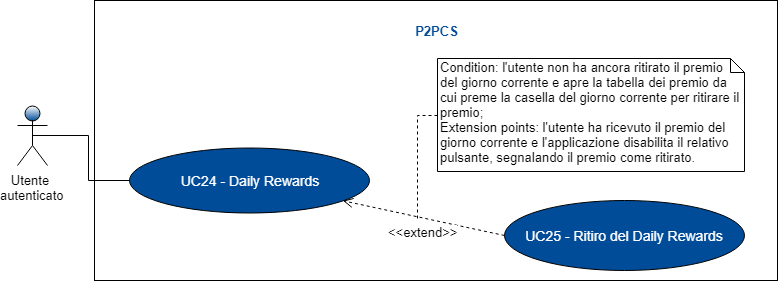
\includegraphics[width=13.2cm]{res/images/UC24Daily.png}
	\centering
	\caption{UC24 - Daily Rewards}
\end{figure}
\subsubsection{UC24 - Daily rewards}
\begin{itemize}
	\item \textbf{Attori Primari}: utente autenticato;
	\item \textbf{Descrizione}: l'applicazione rende disponibile una tabella che illustra i premi giornalieri del mese corrente. La tabella è organizzata sotto forma di calendario, in cui associa ad ogni giorno del mese corrente un premio;
	ogni casella si trova in uno dei seguenti stati:
	\begin{itemize}
		\item 1: il pulsante è disattivato perché il premio non è mai stato ritirato e il giorno a cui è associato non corrisponde con la data corrente;
		\item 2: il pulsante è attivo perché il premio non è mai stato ritirato e il giorno a cui è associato corrisponde con la data corrente;
		\item 3: il pulsante è disattivato e segnalato come già ritirato. 
	\end{itemize} 
	Inoltre, i premi ottenibili possono includere:
	\begin{itemize}
		\item sconti su e-commerce o buoni spesa;
		\item sconto sul prossimo viaggio con \textit{GaiaGo};
		\item viaggio gratuito con \textit{GaiaGo};
		\item accessori per l'auto del minigioco;
		\item bonus di punti esperienza;
		\item oggetti virtuali esclusivi per il minigioco.
	\end{itemize}
	\item \textbf{Scenario principale}: l'utente preme l'icona relativa alla tabella dei Daily Rewards da cui può visualizzare i premi disponibili per il mese corrente e decidere di ritirare il premio del giorno corrente [UC25].
	Ogni premio può essere ritirato solo una volta;
	\item \textbf{Estensioni}: 
		\begin{itemize}
			\item ritiro del premio giornaliero [UC25].
		\end{itemize}
	\item \textbf{Precondizione}: l'utente ha premuto l'icona Daily Rewards;
	\item \textbf{Postcondizione}: l'utente ha visualizzato i premi disponibili per il mese corrente e può aver ritirato il premio del giorno corrente se non lo ha precedentemente fatto [UC25]. 
\end{itemize} 

\subsubsection{UC25 - Ritiro del daily rewards}
\begin{itemize}
	\item \textbf{Attori Primari}: utente autenticato;
	\item \textbf{Descrizione}: l'applicazione rende disponibile dei premi giornalieri, illustrati e ritirabili tramite la tabella Daily Rewards;
	\item \textbf{Scenario principale}: l'utente sta visualizzando la tabella dei premi giornalieri e preme la casella del premio del giorno corrente per ritirarlo;
	\item \textbf{Precondizione}: l'utente non ha ancora ritirato il premio del giorno corrente e apre la tabella dei premio da cui preme la casella del giorno corrente per ritirare il premio;
	\item \textbf{Postcondizione}: l'utente ha ricevuto il premio del giorno corrente e l'applicazione disabilita il relativo pulsante, segnalando il premio come ritirato. 
\end{itemize} 